\begin{definition}[wohl-separiert]
   	\label{def:wellsep}
   	Seien $s > 0$ und $A$ und $B$ zwei endliche Mengen von Punkten in $\R^d$. 
   	$A$ und $B$ heißen \emph{wohl-separiert bezüglich $s$} (engl. well-separated), falls es zwei disjunkte Bälle $C_A$ und $C_B$ gibt, die denselben Radius $R$ haben, sodass $A \subseteq C_A$ und $B \subseteq C_B$ und die euklidische Distanz zwischen den Rändern von $C_A$ und $C_B$ mindestens $s\cdot R$ beträgt.

	Eine solche Zahl $s$ nennen wir die \emph{Trennungsrate} der Mengen $A$ und $B$.
\end{definition}

Das folgende Lemma hält zwei wichtige Eigenschaften von zwei bezüglich $s$ wohl-separierten Mengen $A$ und $B$ fest.
\begin{lemma}
   	\label{lem:wellsep}
	Seien $a, a' \in A$ und $b, b' \in B$. Dann gilt:
	\begin{enumerate}
		\item $\displaystyle |aa'| \leq \frac{2}{s}\cdot|a'b'|$.
		\item $\displaystyle |a'b'| \leq (1+\frac{4}{s})\cdot|ab|$.
	\end{enumerate}
\end{lemma}
\begin{proof}
   	Zu 1. Ist $R$ der Radius von $C_A$ und $C_B$, so gilt $|aa'| \leq 2 \cdot R$. Da $A$ und $B$ wohl-separiert sind, gilt zudem $|a'b'| \geq s \cdot R$, was äquivalent ist zu $R \leq \frac{|a'b'|}{s}$. Durch Einsetzen folgt dann die Behauptung.
   	
   	Zu 2. Da $A$ und $B$ bezüglich $s$ wohl-separiert sind und $C_A$ und $C_B$ beide denselben Radius $R$ haben, gilt $|a'b'| \leq s \cdot R + 4 \cdot R$. Ausklammern rechts ergibt $(1 + \frac{4}{s}) \cdot s \cdot R$. Da ja auch $s \cdot R \leq |ab|$, folgt durch Einsetzen die Behauptung.
\end{proof}

\begin{definition}[WSPD]
   	\label{def:wspd}
   	Sei $S \subseteq \R^d$ und $s > 0$. 
   	Eine Menge $ \{(A_1, B_1), (A_2, B_2), \mathellipsis, (A_m, B_m)\}$ (im Folgenden auch $\{(A_i, B_i)\}_{1 \leq i \leq m}$) von Paaren von nicht-leeren Teilmengen von S ist genau dann eine \emph{Zerlegung in wohl-separierte Paare (engl. well-separated pair decomposition; WSPD)}, wenn für alle $1 \leq i \leq m$ gilt:
   	\begin{enumerate}[label={(\arabic*)}, itemsep=0mm]
   		\item $A_i \cap B_i = \emptyset$.
   		\item Für alle $p, q \in S$ gibt es genau einen Index $1 \leq j \leq m$, sodass entweder $p \in A_j$ und $q \in B_j$ oder $q \in A_j$ und $p \in B_j$.
   		\item $A_i$ und $B_i$ sind bezüglich $s$ wohl-separiert.
   	\end{enumerate}
\end{definition}

\noindent $m$ nennen wir dabei die \emph{Größe} der WSPD.

Die WSPD bildet eine wichtige Grundlage für die beiden Algorithmen, die wir im Folgenden betrachten werden. 
Callahan und Kosaraju haben in \cite{callahan} gezeigt, dass man zu einer gegebenen Menge $L \subset \R^d$ der Größe $n$ eine WSPD  der Größe $m = O(s^dn)$ in $O(n\log n + s^dn)$ Zeit berechnen kann. 
Dabei wird zunächst in $O(n \log n)$ ein sogenannter \emph{(fairer) Split-Tree} berechnet. 
Bei diesem handelt es sich um einen binären Baum, in dessen Blättern die Werte der Grundmenge $S$ in von links nach rechts aufsteigend sortierter Reihenfolge gespeichert sind. 
Aus dem Split-Tree kann dann in $O(s^dn)$ Zeit eine WSPD erstellt werden. 
Wir werden sehen, dass es für unsere Anwendung genügt, eine WSPD für Mengen von Punkten aus $\R$ zu erstellen. 
Für diesen eindimensionalen Fall kann ein fairer Split-Tree mit Hilfe eines einfachen Algorithmus berechnet werden (Abb. \ref{fig:splittree}).

\begin{figure}[b]
	\centering
	\begin{minipage}{.8\linewidth}
		\scriptsize
		\begin{algorithmic}[H]
			\STATE \texttt{compute\_split\_tree(i, j)}  \{
			\begin{ALC@g}
				\IF{$i = j$}
					\STATE erstelle neuen Knoten $u$;
					\STATE speichere das Intervall $[i,i]$ zu $u$;
					\RETURN $u$
				\ELSE
					\STATE $z \coloneqq (S[i] + S[j]) / 2$;
					\STATE $k \coloneqq \text{Index eines Elementes von } S \text{, sodass } S[k] \leq z < S[k+1]$;
					\STATE $v \coloneqq \texttt{compute\_split\_tree(i, k)}$;
					\STATE $w \coloneqq \texttt{compute\_split\_tree(k+1, j)}$;
					\STATE erstelle neuen Knoten $u$;
					\STATE speichere das Intervall $[i, j]$ zu $u$;
					\STATE mache $v$ zum linken Kind von $u$;
					\STATE mache $w$ zum rechten Kind von $u$;
					\RETURN $u$
				\ENDIF
			\end{ALC@g}
			\STATE \}
		\end{algorithmic}
	\end{minipage}
	\caption{Algorithmus zum Erstellen eines fairen Split-Trees zu einer gegebenen Menge $S$ (nach \cite{gudmundsson})}
	\label{fig:splittree}
\end{figure}



Sei $S$ nun eine endliche Teilmenge von $\R$ und $|S| = n$. 
Wir können davon ausgehen, dass uns diese Menge sortiert in einem Array $S[1..n]$ vorliegt und werden später sehen, dass das bei unserem Algorithmus auch tatsächlich der Fall ist. 
Sei $T$ der Split-Tree, der durch das Ausführen von \texttt{compute\_split\_tree(1, n)} entstanden ist.
Für jeden inneren Knoten $k$, also für jeden Knoten, der kein Blatt ist, wird in \texttt{compute\_split\_tree()} zusätzlich das kleinste Intervall der Indizes der Elemente gespeichert, die die Blätter des von $k$ induzierten Teilbaumes bilden.
Die Wurzel speichert also zum Beispiel das Intervall $[1, n]$ und das $i$-te Blatt das Intervall $[i, i]$.
Da $T$ $n$ Blätter hat, erstellen wir insgesamt $O(n)$ Knoten. 
Dabei müssen wir aber für die Bestimmung von $k$ jedes Mal eine Binärsuche durchführen, die $O(\log n)$ Zeit kostet. 

\begin{figure}
   	\makebox[\textwidth][c]{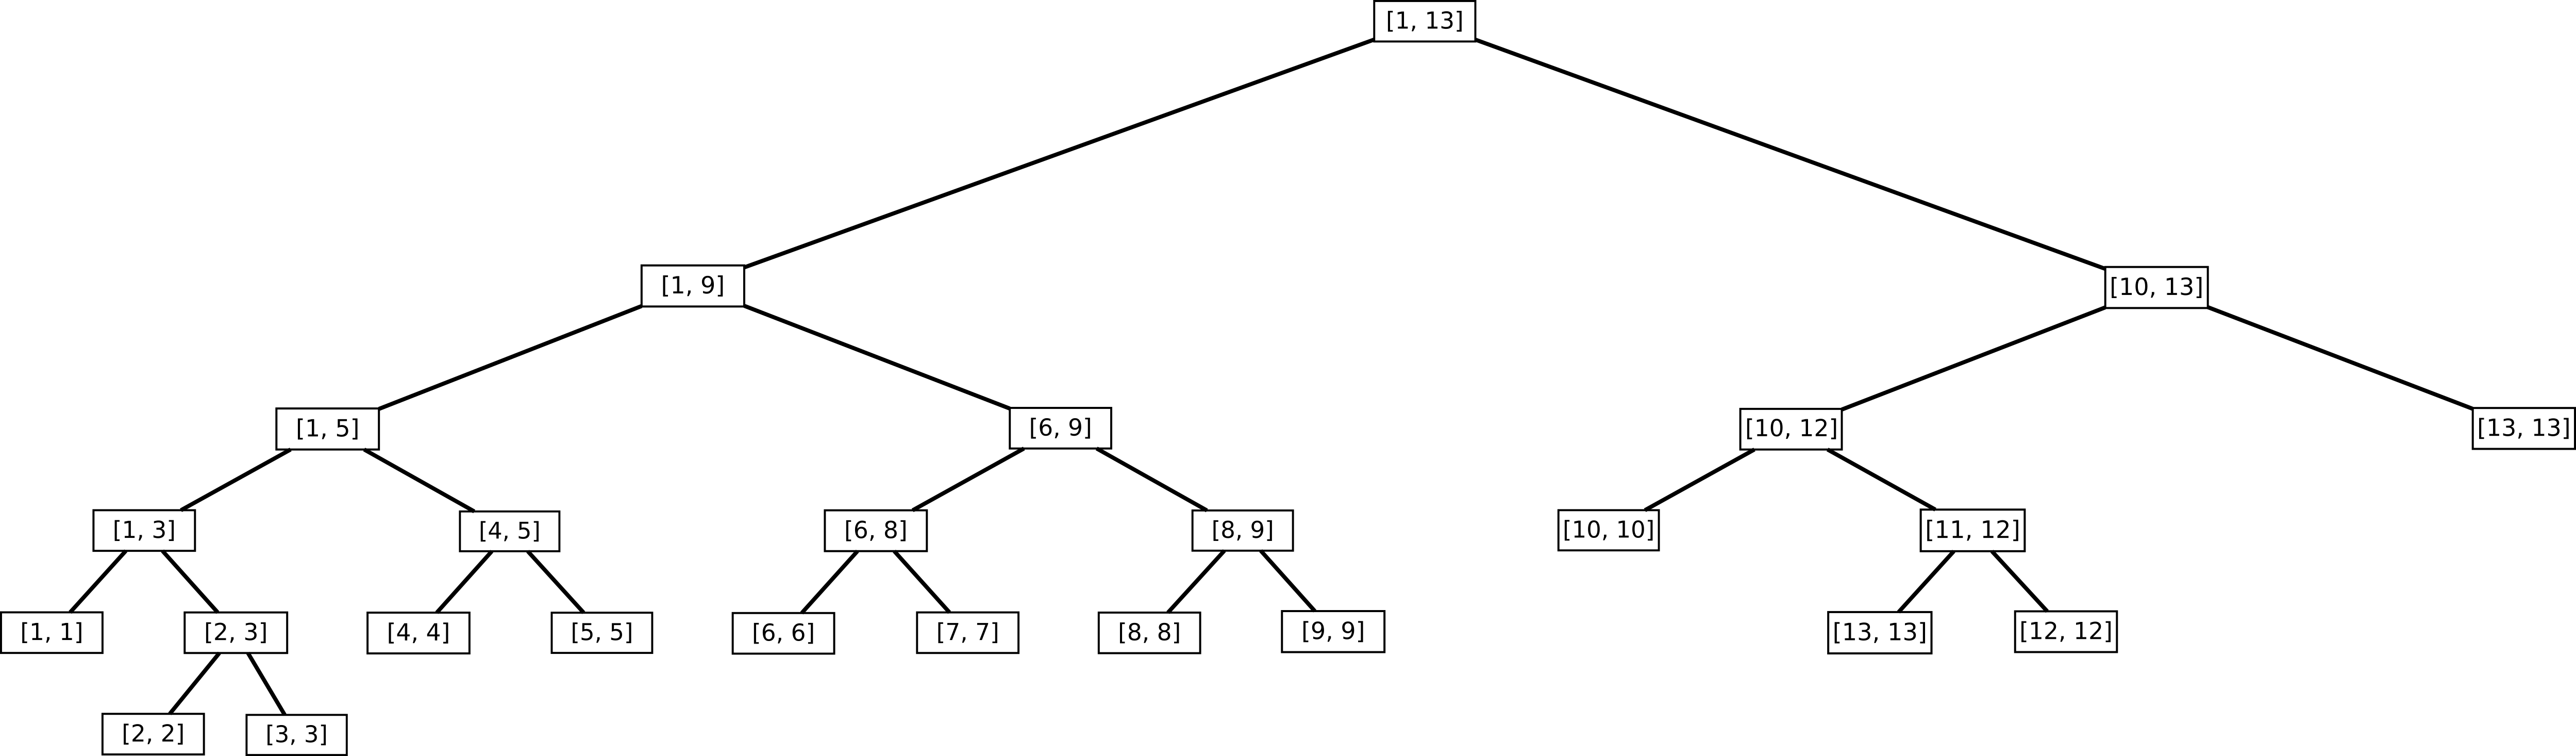
\includegraphics[width=1\textwidth]{split_tree}}
   	\caption{Fairer Split-Tree für die Menge $S=[0.0, 5.0, 9.1, 17.2, 32.2, 37.6, 44.3, 54.3, 67.9, 81.0, 95.4, 96.4, 141.5]$. Die Knoten des Baumes sind mit dem Intervall beschriftet, das mit ihnen gespeichert ist.}
   	\label{fig:splittree}
\end{figure}

Somit ergibt sich für das Erstellen von $T$ eine Gesamtlaufzeit von $O(n\log n)$.
Betrachten wir jetzt zwei innere Knoten $p$ und $q$ von T. Seien $[i, j]$ und $[k, l]$ die Intervalle, die wir mit $p$ und $q$ gespeichert haben und 
\[
R \coloneqq \max(S[j] - S[i], S[l] - S[k]).
\]
Nach Definition \ref{def:wellsep} sind die beiden Intervalle genau dann wohl-separiert, wenn 
\[
S[k] - S[j] \geq R \cdot s \text{ oder } S[i] - S[l] \geq R \cdot s.
\]

\begin{figure}
	\centering
	\begin{minipage}{.8\linewidth}
		\scriptsize
		\begin{algorithmic}[H]
			\STATE \texttt{compute\_wspd(T, s)}  \{
			\begin{ALC@g}
				\STATE \textbf{for each} innerer Knoten $u$ in $T$ \textbf{do}
				\begin{ALC@g}
					\STATE $v \coloneqq \text{ linkes Kind von } u$
					\STATE $w \coloneqq \text{ rechtes Kind von } u$
					\STATE \texttt{find\_pairs(v, w)}
				\end{ALC@g}
			\end{ALC@g}
			\STATE \}
			\STATE \
			\STATE \texttt{find\_pairs(v, w)} \{
			\begin{ALC@g}
				\IF{$S_u$ und $S_v$ sind in Bezug zu $s$ nicht wohl-separiert}
					\STATE Seien $[i, j]$ und $[k, l]$ die Intervalle die mit $u$ bzw. $v$ gespeichert sind;
						\IF{$S[j] - S[i] \leq S[l] - S[k]$}
							\STATE $w_1 \coloneqq \text{ linkes Kind von } w $;
							\STATE $w_2 \coloneqq \text{ rechtes Kind von } w $;
							\STATE \texttt{find\_pairs(v, w\textsubscript{1})};
							\STATE \texttt{find\_pairs(v, w\textsubscript{2})};
						\ELSE
							\STATE $v_1 \coloneqq \text{ linkes Kind von } v $;
							\STATE $v_2 \coloneqq \text{ rechtes Kind von } v $;
							\STATE \texttt{find\_pairs(v\textsubscript{1}, w)};
							\STATE \texttt{find\_pairs(v\textsubscript{2}, w)};
						\ENDIF
				\ELSE
					\STATE Speichere in $u$ und $v$, dass deren Blätter die Teilmengen $A$ und $B$ einer WSPD bilden;
				\ENDIF
			\end{ALC@g}
			
			\STATE \}
		\end{algorithmic}
	\end{minipage}
	\caption{Algorithmus zum Erstellen einer WSPD aus einem gegebenen Split-Tree $T$ und einer Trennungsrate $s$ (nach \cite{gudmundsson})}
	\label{fig:wspd}
\end{figure}

Der in Abbildung \ref{fig:wspd} dargestellte Algorithmus berechnet dann aus dem eben erstellten fairen Split-Tree $T$ eine WSPD.
Betrachten wir diesen nun etwas genauer.
 
Beim Aufruf von \texttt{compute\_wspd(T, s)} werden für jeden Knoten $k$ dessen Kindknoten $v$ und $w$ betrachtet, und dann \texttt{find\_pairs(v, w)} aufgerufen. 
Da die Elemente von $S$ in den Blättern von $T$ gespeichert sind und jedes Element genau durch ein Blatt dargestellt wird, ist klar, dass der linke Kindknoten $v$ und der rechte $w$ disjunkte Teilmengen von $S$ repräsentieren. 
Somit ist Forderung (1) der WSPD erfüllt. \texttt{find\_pairs(v, w)} überprüft, ob die mit $v$ und $w$ gespeicherten Intervalle $S_v$ und $S_w$ wohl-separiert sind; ist dies der Fall, speichern wir mit $v$, dass seine Blätter das Element $A_i$ einer WSPD bilden, und mit $w$, dass seine Kinder das Element $B_i$ darstellen. 
Sind die Intervalle nicht wohl-separiert, steigen wir solange in Richtung des größeren Intervalls im Baum herab, bis wir auf zwei wohl-separierte Intervalle treffen. 
Das ist spätestens dann der Fall, wenn wir zwei Blätter betrachten, denn dann ist $R = 0$.
Wir sehen also, dass die erste und die dritte Forderung der Definition der WSPD durch den Algorithmus erfüllt werden. 
Man kann auch zeigen, dass er die zweite erfüllt, was wir an dieser Stelle allerdings überspringen werden. 
Interessierte können einen vollständigen Beweis auf Seite 72ff in \cite{callahan} nachlesen. Callahan und Kosaraju, die Autoren dieses Artikels, haben auch bewiesen, dass \texttt{compute\_wspd(T, s)} eine zu $T$ gehörende WSPD der Größe $O(sn)$ in $O(sn)$ Zeit berechnet. 
Halten wir also fest:
\begin{theorem}
	\label{theo:wspdtime}
	Sei $S \subset \R$ endlich und $n = |S|$. Dann kann in $O(n \log n + sn)$ Zeit ein Split-Tree $T$ und eine dazugehörige WSPD $\{(A_i, B_i)\}_{1 \leq i \leq m}$ der Größe $m = O(sn)$ berechnet werden.
\end{theorem}